\section{Hardware Specifications}

All experiments were conducted on a high-performance
PC with the following specifications: 

\begin{itemize}
    \item CPU: Intel Core i7-9800X CPU @ 3.80GHz,
    3792 Mhz, 8 core, 16 threads
    \item GPU: 2 NVIDIA RTX 2080 Ti GPU with 12GB
    VRAM each
    \item RAM: 64 GB DDR4
    \item Storage: 1 TB Seagate BarraCuda HDD
\end{itemize}

\section{Software Environment}

The experiments were implemented using the following software stack:

\begin{itemize}
    \item Operating System: Windows 11 Pro
    \item Python: 3.10.14
    \item PyTorch: 2.4.0
    \item CUDA: 12.0
    \item TorchRL: 0.5.0
    \item MuJoCo: 3.14
\end{itemize}

\section{Network Architectures Details}

\subsection{WRe-CTDG Network Structure}

The WRe-CTDG framework consists of three main components:
Encoder $E_u$, Generator $G_s$, and Critic $C$.
Here are the details of each network:\\
\textbf{Encoder $\mathbf{E_u}$:}
\begin{itemize}
    \item Input layer: 2 $\times$ numerical state dimensions
    + 2 $\times$ latent state dimensions + action dimension
    \item Hidden layers: 4 fully connected layers with 256, 512, 512, and 256 units respectively
    \item Output layer: noise dimension + 1 (for reward prediction)
    \item Activation function: ReLU for hidden layers,
    Tanh/Sigmoid/Identity for reward output, Linear for noise output
\end{itemize}
\textbf{Generator $\mathbf{G_s}$:}
\begin{itemize}
    \item Input layer: numerical state dimension
    + latent state dimension + action dimension +
    noise dimension
    \item Hidden layers: 4 fully connected layers
    with 256, 512, 256, and 128 units respectively
    \item Output layer: numerical state dimension
    + latent state dimension
    \item Activation function: ReLU for hidden layers,
    Linear for output layer
\end{itemize}
\textbf{Critic $\mathbf{C}$:}
\begin{itemize}
    \item Input layer: 2 $\times$ numerical state dimensions
    + 2 $\times$ latent state dimensions + action dimension
    + noise dimension
    \item Hidden layers: 4 fully connected layers with 256,
    512, 256, and 128 units respectively
    \item Output layer: 1
    \item Activation function: ReLU
    for hidden layers, Linear for output layer
\end{itemize}
For environments with image inputs, we additionally used a
Convolutional AutoEncoder architecture to
encode and decode the state representations:\\
\textbf{Convolutional Encoder:}
\begin{itemize}
    \item 5 downsampling blocks
    \item Each block contains 2-3 convolutional layers
    with BatchNorm and ReLU activation
    \item Number of filters increases progressively:
    $$ in\_channels \rightarrow base \rightarrow 2
    \times base \rightarrow 4\times base \rightarrow
    8\times base \rightarrow 16\times base $$
    with $base = 8$.
    \item MaxPool2D with kernel size $2\times 2$ and stride
    2 for downsampling between blocks
    \item Final $1\times 1$ convolutional layer to
    reduce channel dimension to $bn = 1$ (bottleneck)
\end{itemize}
\textbf{Convolutional Decoder:}
\begin{itemize}
    \item Initial $1\times 1$ convolutional layer 
    to expand channel dimension from $bn$ to $16 \times base$
    \item 5 upsampling blocks
    \item Each block contains 2-3 convolutional
    layers with BatchNorm and ReLU activation
    \item Number of filters decreases progressively:
    $$ 16\times base \rightarrow 8
    \times base \rightarrow 4\times base \rightarrow
    2\times base \rightarrow base \rightarrow in\_channels$$
    with $base = 8$.
    \item Upsampling using transposed convolution
     with kernel size $2\times 2$ and stride 2
    \item Final layer uses Tanh activation
\end{itemize}
The encoder and decoder are symmetric, with the number of filters changing at each level.

\subsection{S-CTDG Network Structure}

The S-CTDG framework for \textbf{images} employs a network architecture
consisting of two components: a convolutional U-Net for counterfactual
image generation
and a separate convolutional network with a fully connected head for
reward prediction.\\
\textbf{U-Net}:
\begin{itemize}
    \item 5 downsampling blocks and 5 upsampling blocks
    \item Each block contains 2-3 convolutional layers
    with BatchNorm and ReLU activation
    \item Number of filters increases
    progressively in downsampling:
    $$ in\_channels \times (1 + stack\_length) + 2 \times (action\_channels)
    \rightarrow $$$$\rightarrow base \rightarrow 2
    \times base \rightarrow 4\times base \rightarrow
    8\times base \rightarrow 16\times base $$
    where the first term is the stack of current and previous images
    concatenated along the channel dimension with the next state image
    and the action and counterfactual action images.
    The number of filters then decreases in upsampling:
    $$ 16\times base \times 2 \rightarrow 8 \times base \times 2 \rightarrow
    4\times base \times 2\rightarrow$$ $$ \rightarrow 2\times base \times 2
    \rightarrow base \times 2 \rightarrow in\_channels$$
    with $base = 64$, in upsampling the filters are doubled
    since we concatenate the corresponding downsampling block.
    \item Convolution with kernel size $3\times 3$, stride 1,
    and padding 1
    \item MaxPool2D with kernel size $2\times 2$ and stride
    2 for downsampling between blocks
    \item Final layer uses a Softsign activation function
\end{itemize}
\textbf{Reward Prediction Network}:
\begin{itemize}
    \item 5 downsampling blocks
    \item Each block contains 2-3 convolutional layers
    with BatchNorm and ReLU activation
    \item Number of filters increases
    progressively in downsampling:
    $$ in\_channels \times (1 + stack\_length) + action\_channels
    \rightarrow base \rightarrow$$$$\rightarrow 2
    \times base \rightarrow 4\times base \rightarrow
    8\times base \rightarrow 16\times base $$
    where the first term is the stack of current and previous images
    concatenated along the channel dimension with the
    estimated counterfactual next state image
    and the counterfactual action image.
    As before, $base = 64$.
    \item Convolution with kernel size $3\times 3$, stride 1,
    and padding 1
    \item MaxPool2D with kernel size $2\times 2$ and stride
    2 for downsampling between blocks
    \item Final layer uses an Identity activation function
\end{itemize}

The S-CTDG framework for \textbf{numerical} data
employs a network architecture consisting of a single
fully connected network branched into two heads:
one for counterfactual data generation
and one for reward prediction.
The network architecture is as follows:
\begin{itemize}
    \item Input layer: 2 $\times$ numerical state dimensions
    $ + $ $2 \times $ action dimension
    \item Hidden layers: 7 fully connected layers with
    512, 512, 512 and 256 units respectively
    \item Output layer for counterfactual data generation:
    numerical state dimension, Linear activation function
    \item Output layer for reward prediction: 1,
    Identity activation function
\end{itemize}

\subsection{Reinforcement Learning Algorithms (D3QN and TD3)}

For the reinforcement learning algorithms, we used the following architectures:\\
For discrete action spaces we used \textbf{D3QN:}
\begin{itemize}
    \item Input layer: state dimension
    \item Hidden layers: 4 fully connected layers with 32, 64, 128 and 128
    units respectively
    \item Output layer: action dimension
\end{itemize}
It is a \textbf{Dueling CNN DQNetwork} as presented in \cite{d3qn}.\\
Then, for continuous action spaces we used \textbf{TD3:}\\
Actor:
\begin{itemize}
    \item Input layer: state dimension
    \item Hidden layers: 3 fully connected layers with 32, 64, 128 and 128
    units respectively
    \item Output layer: action dimension
    \item Activation function: ReLU for hidden layers, Tanh for output layer
\end{itemize}
Critic:
\begin{itemize}
    \item Input layer: state dimension + action dimension
    \item Hidden layers: 3 fully connected layers with 32, 64, 128 and 128
    units respectively
    \item Output layer: 1
    \item Activation function: ReLU for hidden layers, Linear for output layer
\end{itemize}
The actor and critic networks are modelled after
the architectures presented in \cite{lillicrap2019}. 

\section{Experimental Setup}

\subsection{Dataset Collection}

For each environment, we collected a dataset of transitions using a random policy.
This dataset served as the basis for our counterfactual
data generation and reinforcement learning experiments.

The number of transitions in the dataset was different for each environment:
\begin{itemize}
    \item Acrobot: 20'000 transitions, observation stack length: 2
    \item Half Cheetah: 50'000 transitions, observation stack length: 4
    \item Ant: 50'000 transitions, observation stack length: 4
    \item Diabetes: 100 transitions, observation stack length: 1
\end{itemize} 

\subsection{Convolutional AutoEncoder Training}

We trained the CAE with each one of the three different image-based
environments: Acrobot, Half Cheetah, and Ant.
For this task we employed the Adam optimizer
(Learning Rate: $1\times 10^{-4}$, $\beta_1$: 0.5, $\beta_2$: 0.9)
and a batch size of 128. The model was trained for 10'000 iterations
on the combined dataset from all three environments. We used the standard
MSE loss for the reconstruction error with a weight mask
to give less importance to the background pixels.

\subsection{Counterfactual Data Generation}

We used both WRe-CTDG and S-CTDG frameworks to generate counterfactual data.
The augmentation factor $\alpha$ was set to 4, effectively quadrupling
the size of the original datasets,
except on the Diabetes environment where $\delta = 8$ was used.
Only a subset of the original dataset
was used for generating counterfactual data.

Training parameters:
\begin{itemize}
    \item Batch size: 32
    \item Optimizer: Adam (learning rate: $1\times 10^{-4}$, $\beta_1$: 0.5, $\beta_2$: 0.9)
    \item Number of iterations: 10'000 for WRe-CTDG, 100'000 for S-CTDG\\
    (both $\approx 12$h of training)
    \item Frame size for image-based environments: $128\times 128$
\end{itemize}
Size of the augmented datasets:
\begin{itemize}
    \item Acrobot: 10'000 $\times \, \alpha =$ 40'000 transitions 
    \item Half Cheetah: 10'000 $\times \, \alpha =$ 40'000 transitions
    \item Ant: 10'000 $\times \, \alpha =$ 40'000 transitions
    \item Diabetes: 20 $\times \, \delta =$ 160 transitions
\end{itemize}

We measured the Mean Absolute Error (MAE) on a validation set
between the generated counterfactual states and the ground truth
states after the training of WRe-CTDG (comparison between encoded values)
and S-CTDG (comparison between images) frameworks.

\subsection{Reinforcement Learning Training}

We trained D3QN and TD3 algorithms on both the original and augmented datasets.
The training process involved:
\begin{itemize}
    \item Number of training steps: 1'000 for Acrobot, 2'000 for Half Cheetah, 3'000 for Ant, 8'000 for Diabetes
    \item Batch size: 256
    \item Discount factor ($\gamma$): 0.99
    \item Optimizer: Adam (Learning Rate: $1\times 10^{-4}$, $\beta_1$: 0.0, $\beta_2$: 0.9)
    \item Exploration strategy: $\epsilon$-greedy with decay factor $\tau = 0.005$
\end{itemize}
Training progress was monitored through periodic evaluations
of the policy within the environment.
The evaluation metric employed for comparisons was the best
reward achieved over all evaluation episodes. 

\section{Results}

\subsection{Convolutional Autoencoder Results}

Table \ref{tab:reconstruction_mse} presents the mean squared error (MSE) of the reconstruction loss for each environment after training:

\begin{table}[h]
    \centering
    \begin{tabular}{@{}lc@{}}
        \toprule
        \textbf{Environment} & \textbf{Reconstruction MSE} \\ \midrule
        Acrobot              & 1.364                       \\
        Half Cheetah         & 13.539                      \\
        Ant                  & 14.294                      \\ \bottomrule
    \end{tabular}
    \caption{Mean Squared Error (MSE) of reconstruction loss for each environment}
    \label{tab:reconstruction_mse}
\end{table}

The CAE achieved a significantly lower reconstruction error on
the Acrobot environment compared to Half Cheetah and Ant.
This substantial difference in reconstruction capability is likely due
to the simpler visual structure of Acrobot, while Half Cheetah and Ant
present more complex visual features and dynamics.

While a successful Acrobot reconstruction is shown
in Figure \ref{fig:acrobot_recon},
the poor reconstruction capability for Half Cheetah and Ant
is visually demonstrated in Figures \ref{fig:half_cheetah_recon} and
\ref{fig:ant_recon}, respectively.

\begin{figure}[h]
    \centering
    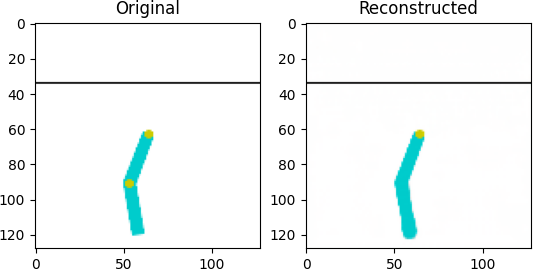
\includegraphics[width=.6\textwidth]{figures/ch5/ae_acrobot.png}
    \caption{Acrobot Reconstruction}
    \label{fig:acrobot_recon}
\end{figure}

\begin{figure}[h]
    \centering
    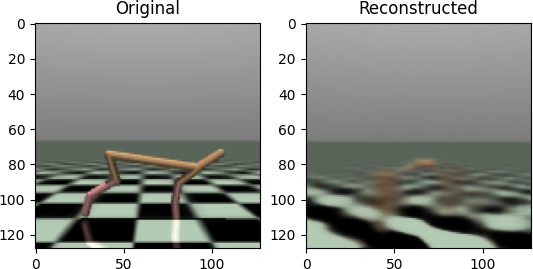
\includegraphics[width=.6\textwidth]{figures/ch5/ae_half_cheetah.png}
    \caption{Half Cheetah Reconstruction}
    \label{fig:half_cheetah_recon}
\end{figure}

\begin{figure}[h]
    \centering
    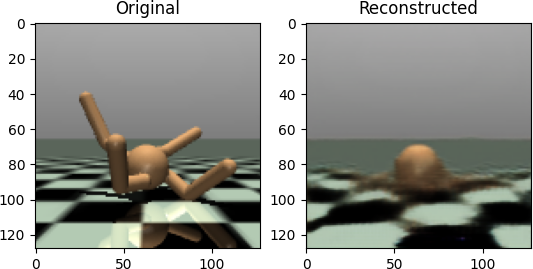
\includegraphics[width=.6\textwidth]{figures/ch5/ae_ant.png}
    \caption{Ant Reconstruction}
    \label{fig:ant_recon}
\end{figure}

These results indicate that while the CAE successfully learned to
encode and reconstruct images from all three environments,
its performance varied significantly across them. The high
reconstruction errors and poor visual quality for Half Cheetah
and Ant suggest that the current CAE architecture may not be
optimal for capturing the complex visual features of these environments.
This limitation, as we will see, could have potentially impacted the effectiveness
of using these learned latent representations in the subsequent reinforcement
learning algorithms, particularly for the more visually complex environments.

\subsection{Reconstruction Loss During Generation}

The MAE values on the validation sets
between the generated counterfactual states and the ground truth
states for both frameworks
are shown in Table \ref{tab:mae}.

\begin{table}[h]
    \centering
    \begin{tabular}{@{}lcccc@{}}
    \toprule
    \multicolumn{1}{c}{\multirow{2}{*}{\textbf{Environment}}} & \multicolumn{2}{c}{\textbf{WRe-CTDG MAE}}   & \multicolumn{2}{c}{\textbf{S-CTDG MAE}}     \\ \cmidrule(l){2-5} 
    \multicolumn{1}{c}{}                                      & \textit{States Loss} & \textit{Reward Loss} & \textit{States Loss} & \textit{Reward Loss} \\ \midrule
    Acrobot                                                   & 0.25189              & 0.04523              & 0.00147              & 0.04821              \\
    Half Cheetah                                              & 0.22064              & 0.06564              & 0.03946              & 0.05912              \\
    Ant                                                       & 0.27296              & 0.06289              & 0.09391              & 0.07071              \\
    Diabetes                                                  & 0.24343              & 0.07265              & 0.12710              & 0.07582              \\ \bottomrule
    \end{tabular}
    \caption{WRe-CTDG and S-CTDG Reconstruction Loss}
    \label{tab:mae}
\end{table}

The S-CTDG framework demonstrates superior reconstruction
capabilities across all the image-based environments,
as evidenced by the lower MAE values.
To visually illustrate these reconstruction capabilities, we present a
series of figures comparing original images to their S-CTDG reconstructions
for each environment.

Figure \ref{fig:acrobot_recon} showcases the S-CTDG reconstruction
for the Acrobot environment. The remarkably low MAE
is reflected in the near-perfect visual fidelity of the reconstructed image,
with virtually no discernible differences from the original.

\begin{figure}[h]
    \centering
    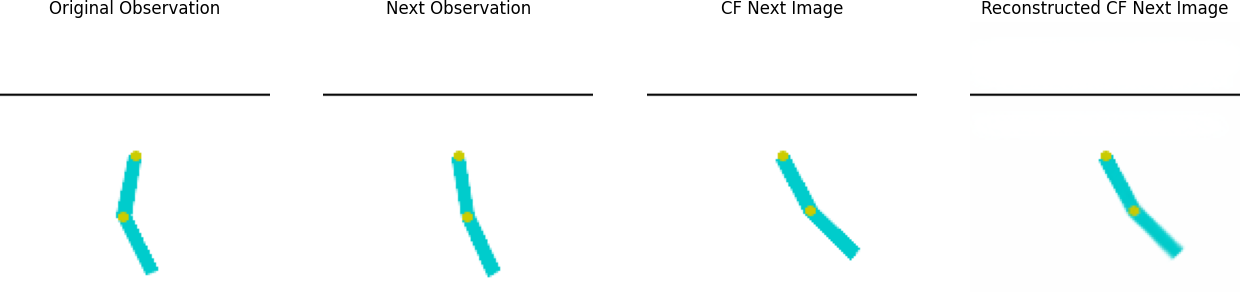
\includegraphics[width=\textwidth]{figures/ch5/e2e_acro.png}
    \caption{S-CTDG results for the Acrobot environment}
    \label{fig:acrobot_recon}
\end{figure}

The Half Cheetah environment reconstruction,
shown in Figure \ref{fig:half_cheetah_recon},
demonstrates the S-CTDG's ability to capture complex articulated structures.
With a MAE of 0.03946, the reconstruction still maintains
the overall structure and positioning of the ant, with some loss of
sharpness in the finer details of the legs and joints.

\begin{figure}[H]
    \centering
    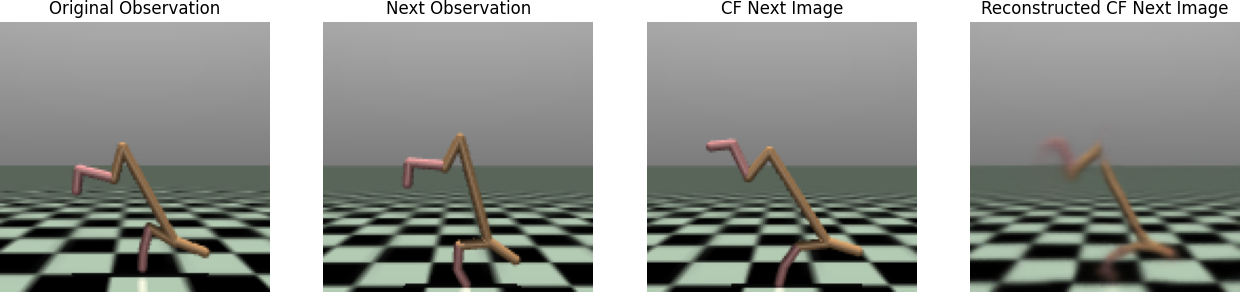
\includegraphics[width=\textwidth]{figures/ch5/e2e_half.png}
    \caption{S-CTDG results for the Half Cheetah environment}
    \label{fig:half_cheetah_recon}
\end{figure}

Figure \ref{fig:ant_recon} illustrates the S-CTDG reconstruction
for the Ant environment. Despite the higher MAE of 0.09391 compared
to the previous environments, the reconstruction still captures
the essential features of the ant's body and limbs, albeit with
some loss of detail and sharpness.

\begin{figure}[H]
    \centering
    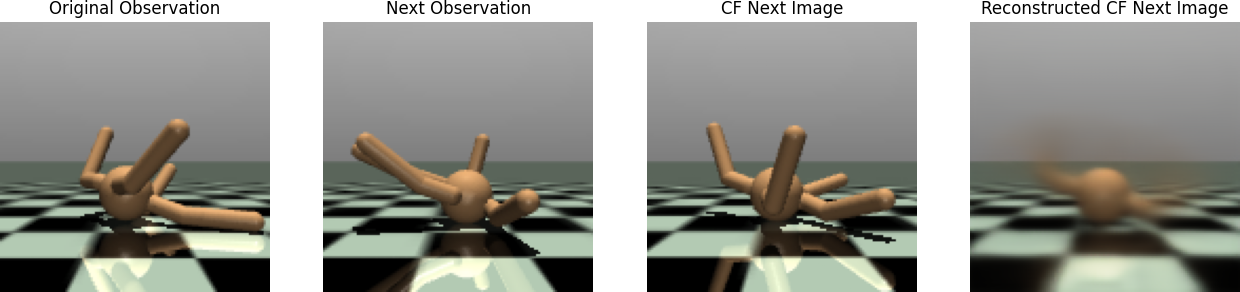
\includegraphics[width=\textwidth]{figures/ch5/e2e_ant.png}
    \caption{S-CTDG results for the Ant environment}
    \label{fig:ant_recon}
\end{figure}

For the Diabetes environment, as it doesn't involve image data,
we do not provide a visual representation. However, it's worth noting
that even here the S-CTDG outperforms the WRe-CTDG 
in terms of MAE.

\subsection{Reinforcement Learning Performance}

We evaluated the performance of D3QN and TD3 algorithms on both the
original and augmented datasets. The results are presented
in Table \ref{tab:rl_reward}: the reward value shown is the best reward
over all the evaluation episodes.

\begin{table}[H]
    \centering
    \begin{tabular}{@{}llccc@{}}
        \toprule
        \textbf{Environment} & \textbf{Algorithm} & \textbf{No Aug.} & \textbf{WRe-CTDG Aug.} & \textbf{S-CTDG Aug.} \\ \midrule
        Acrobot              & D3QN               & -57.47           & -55.90                 & -53.35               \\
        Half Cheetah         & TD3                & 8.19             & 74.13                  & 256.09                \\
        Ant                  & TD3                & 27.06            & 25.28                  & 168.54                 \\
        Diabetes             & D3QN               & 0.04             & 0.06                   & 0.12                   \\ \bottomrule
    \end{tabular}
    \caption{Reinforcement Learning Best Reward Value}
    \label{tab:rl_reward}
\end{table}

In Figure \ref{fig:rew_acrobot} we show the reward trends for the
Acrobot environment using D3QN,
in the case of Half Cheetah, we show the reward trends in
Figure \ref{fig:rew_cheetah},
the trends of reward values for the Ant environment
are shown in Figures \ref{fig:rew_ant} and,
at last, the reward trends for the Diabetes environment are shown in
Figures \ref{fig:rew_diabetes}.

\begin{figure}[H]
    \centering
    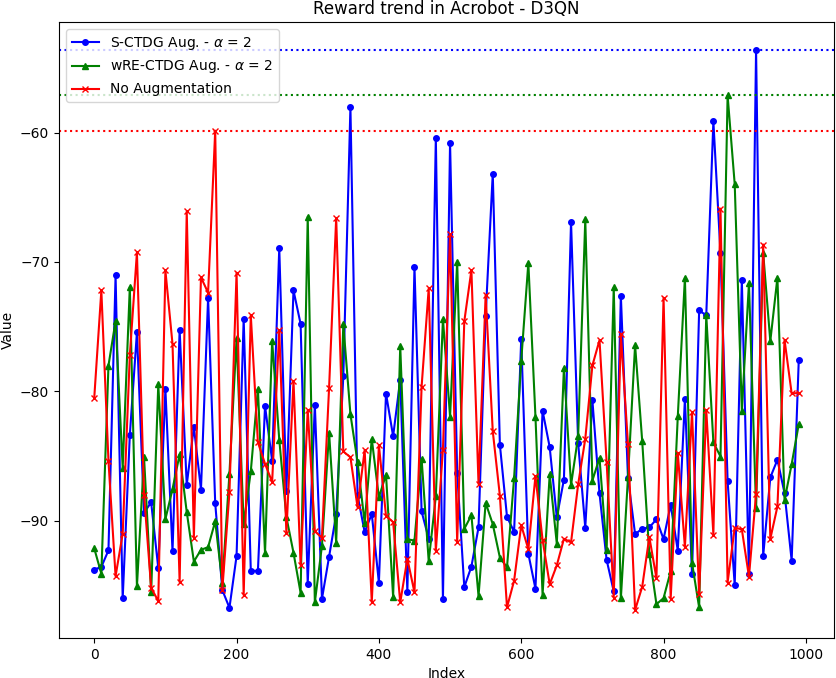
\includegraphics[width=.8\textwidth]{figures/ch5/rew_acrobot.png}
    \caption{Acrobot Reward Trends}
    \label{fig:rew_acrobot}
\end{figure}

\begin{figure}[H]
    \centering
    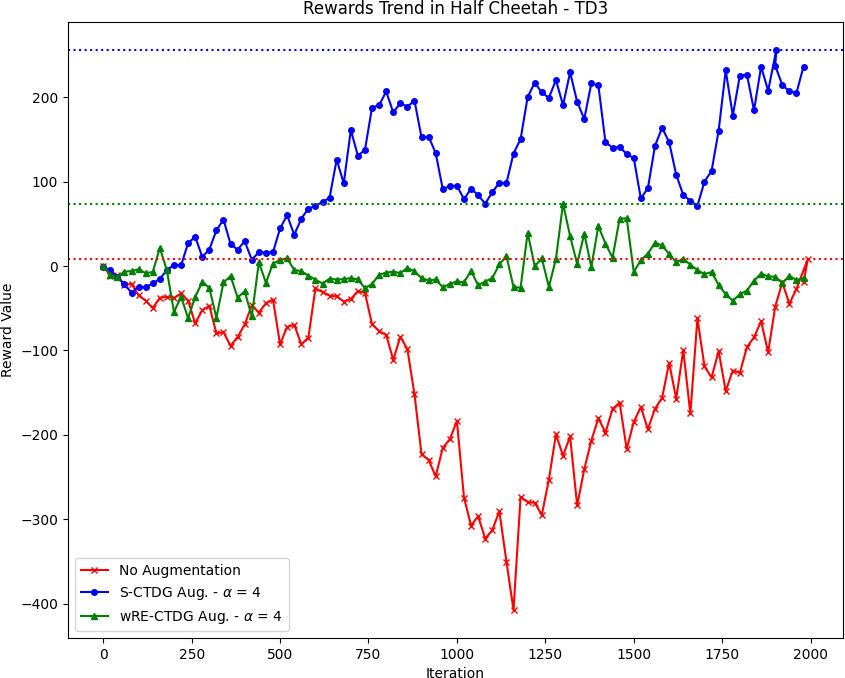
\includegraphics[width=.8\textwidth]{figures/ch5/rew_halfcheetah.png}
    \caption{Half Cheetah Reward Trends}
    \label{fig:rew_cheetah}
\end{figure}

\begin{figure}[H]
    \centering
    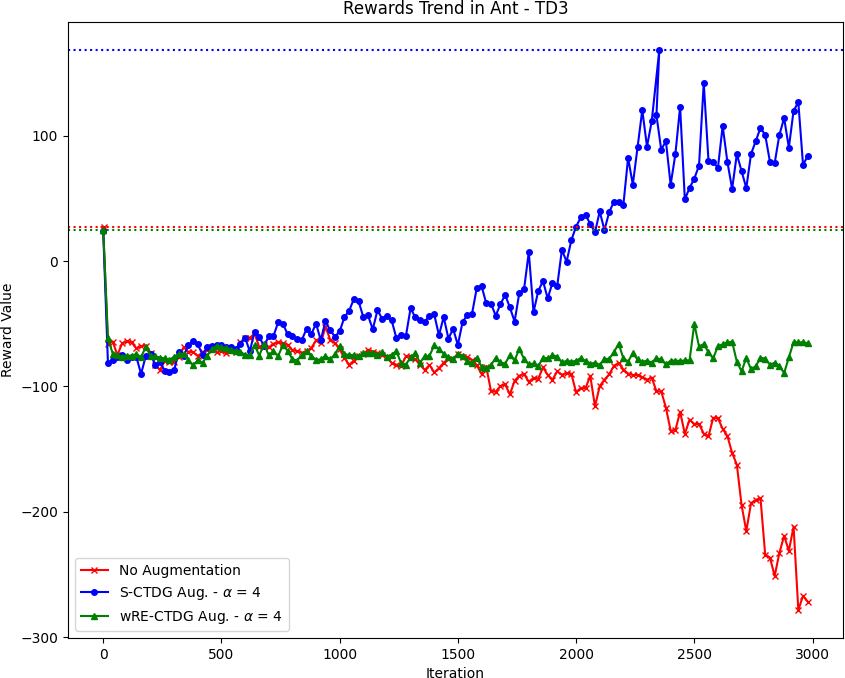
\includegraphics[width=.8\textwidth]{figures/ch5/rew_ant.png}
    \caption{Ant Reward Trends}
    \label{fig:rew_ant}
\end{figure}

\begin{figure}[H]
    \centering
    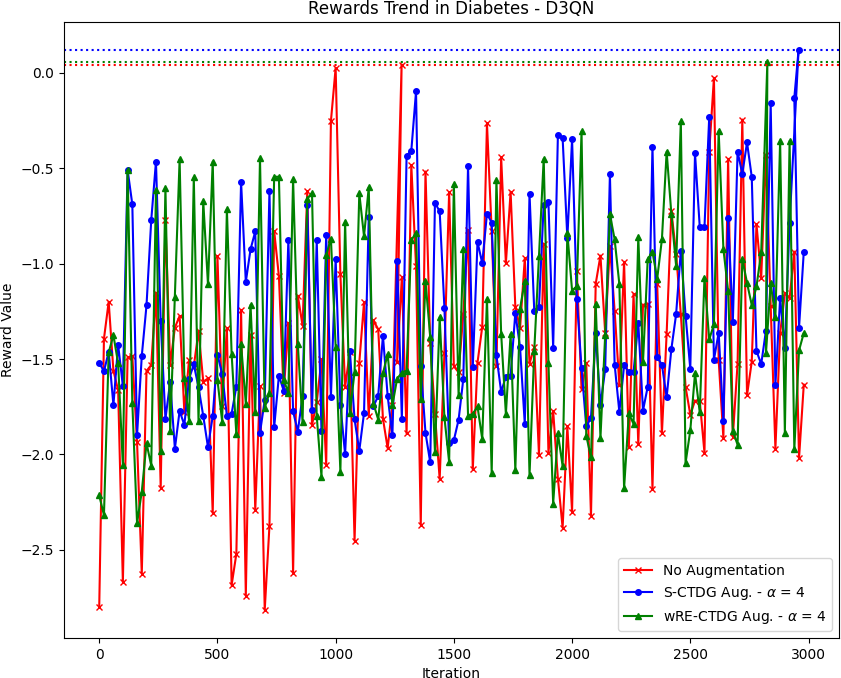
\includegraphics[width=.8\textwidth]{figures/ch5/rew_diabetes.png}
    \caption{Diabetes Reward Trends}
    \label{fig:rew_diabetes}
\end{figure}

\section{Discussion and Analysis of Results}

These findings underscore the potential of counterfactual data generation,
especially S-CTDG, in enhancing the performance of reinforcement learning
algorithms across a variety of tasks and environments.

However, it is important to note that the effectiveness of S-CTDG
comes with significant prerequisites and limitations:
\begin{enumerate}
    \item \textbf{Prior knowledge of system noise:} S-CTDG requires prior
    knowledge of the noise affecting the system.
    This assumption may not always hold in real-world scenarios,
    where the exact nature and distribution of noise might be
    unknown or difficult to model accurately.
    \item \textbf{Ability to perform counterfactual actions:} The S-CTDG
    method necessitates the ability to perform counterfactual actions during
    the data collection process. This requirement can be challenging or
    even impossible to meet in certain environments, particularly in
    real-world applications where data collection might be constrained
    by physical limitations, safety concerns, or ethical considerations.
\end{enumerate}
These constraints highlight an essential trade-off: while S-CTDG
demonstrates superior performance in our experiments,
its applicability may be limited to scenarios where we have
detailed knowledge of the system dynamics and full control over
the data collection process. In contrast, methods like WRe-CTDG,
while generally less effective, may be more broadly applicable as
they don't impose such strict requirements on the data collection
process or prior knowledge of the system.